\subsection{Crystalline Rock Samples}
\Authors{TU Freiberg}
\todo[inline]{[TUBAF](): Introduction to URL Reiche Zeche}

\subsubsection{URL Reiche Zeche Freiberg}
The Reiche Zeche mine is located close to the city center of Freiberg, Saxony. It operated as a silver mine for several decades and became a part of the TU Freiberg when silver mining was no longer profitable. Nowadays the mine is used as an underground research laboratory (URL) and for teaching purposes. The roughly $4\,\text{km}^2$ sized area is well documented in terms of geology, mineralogy, geophysics and geometry. Draining of the mine is done using the "Rothsch\"onberger Stollen (tunnel)".\\
Due to its long history, the development of new technologies and the importance for the development of the whole region the mining sites and the associated infrastructure are listed as UNESCO world heritage site.\\
Current projects are for example dealing with bio-leaching or complex experiments which study the influence of hydro-fracking experiments on the stress state (STIMTEC project).\\
The Reiche Zeche is equipped with an underground railway system, installed electricity, water and air pressure. The experienced personal and the nearby located mining agency help to successfully conduct experiments in about 150 m depth. 




\subsubsection{Rock material used in the direct shear tests}
\begin{figure}[!ht]
\begin{center}
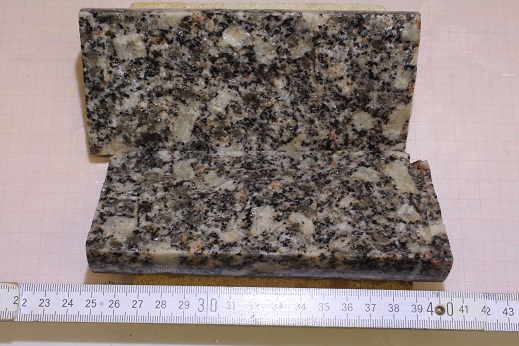
\includegraphics[width=0.5\textwidth]{./figures/ExpRockGranite.JPG}
\end{center}
\caption{Granite sample}
\label{fig:RockGranite}
\end{figure}

\begin{figure}[!ht]
\begin{center}
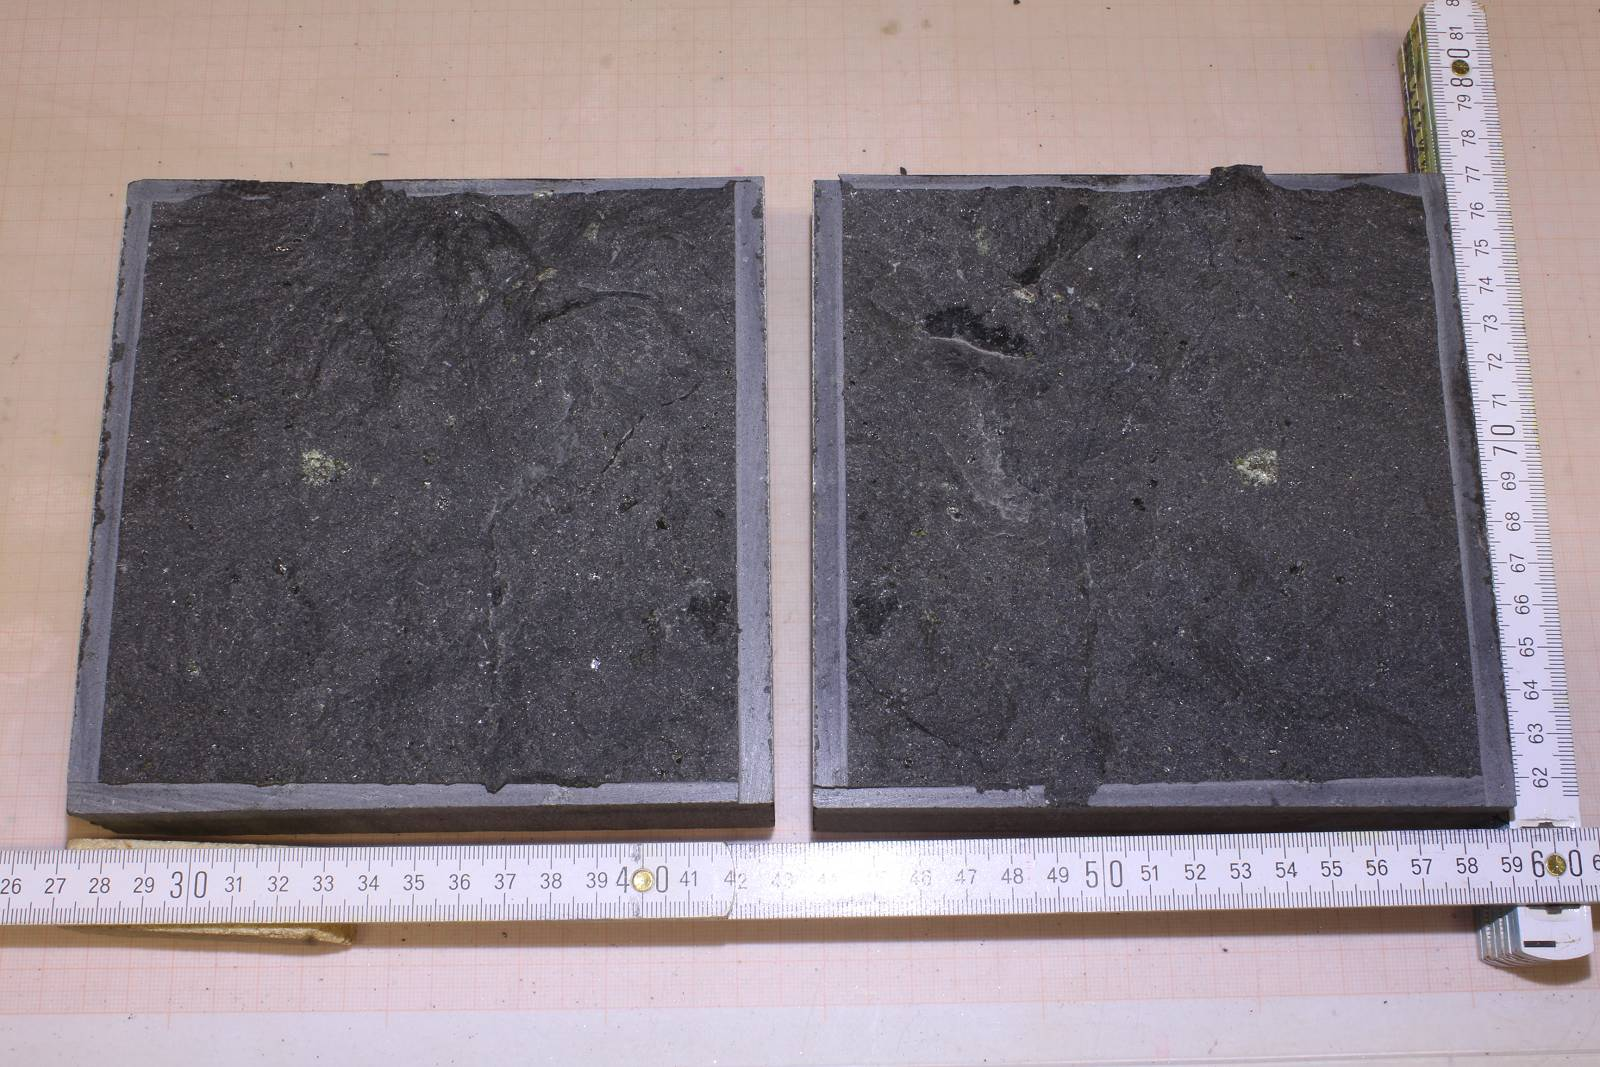
\includegraphics[width=0.5\textwidth]{./figures/ExpRockBasalt.jpg}
\end{center}
\caption{Basalt sample}
\label{fig:RockBasalt}
\end{figure}

Two different crystalline rock types are used. Granite is a coarse-grained intrusive igneous rock. The grains are on the millimetre to centimetre scale, see Fig. \ref{fig:RockGranite}. The typical main minerals of granites are quartz, feldspar and plagioclase.\\
Basalt is an fine-grained extrusive igneous rock. It is rich of plagioclase. See Fig. \ref{fig:RockBasalt}.\\
Lab tests to evaluate basic rock parameters of the intact rock material like elastic constants, compressive strength, cohesion or friction angle have been conducted. The values of the granite and basalt used in the experiments can be found in table \ref{table:MEX7_rockParam}.\\
\begin{table}[!ht]
\begin{center}
\begin{tabular}{l c r r r}
variable & symbol & granite & basalt & unit\\
\hline
density & $\rho$ & $2.59$ &3.06 &$\text{g}/\text{cm}^3$\\
compressive strength & $u_c$ & $120.54$&272.92 &$\text{MPa}   $\\
tensile strength & $u_t$ & $7.02$&16.61 &$ \text{MPa}   $\\
%static elastic modulus & $E_s$ & $50.00$& &$ \text{GPa}   $\\
elastic modulus & $E$ & $49.75$&105.46 &$ \text{GPa}   $\\
Poisson's ratio & $\nu$ & 0.26 & 0.26  & -\\
fracture toughness & $K_I$ & $0.95$& 2.61 &$\text{MPa}\cdot\text{m}^{0.5}$\\
friction angle (Mohr) & $\Phi$ &  $52.5$& 44 &$^\circ$\\
cohesion & $c$ &  $22.5$& 25.00  &$ \text{MPa}   $\\
basic friction angle &$\Phi_b$ &30 & 31.2 & $^\circ$\\
\end{tabular}
\caption{Rock parameters of granite and basalt used in the direct shear tests.}
\label{table:MEX7_rockParam}
\end{center}
\end{table}